\documentclass[a4paper,UTF8]{article}
\usepackage{ctex}
\usepackage[margin=1.25in]{geometry}
\usepackage{color}
\usepackage{graphicx}
\usepackage{amssymb}
\usepackage{amsmath}
\usepackage{amsthm}
%\usepackage[thmmarks, amsmath, thref]{ntheorem}
\theoremstyle{definition}
\newtheorem*{solution}{Solution}
\newtheorem*{prove}{Proof}
\usepackage{multirow}
\usepackage{url}
\usepackage{enumerate}
\usepackage{algorithm}
\usepackage{algorithmic}
\renewcommand{\algorithmicrequire}{\textbf{Input:}}
\renewcommand{\algorithmicensure}{\textbf{Procedure:}}
\renewcommand\refname{参考文献}
\usepackage{graphicx} 
\usepackage{booktabs}  
\usepackage{threeparttable}

%--

%--
\begin{document}
{\flushleft \bf \LARGE 分析结果} 

\section*{数据分布(53522)}
\subsection*{load scores 分布}
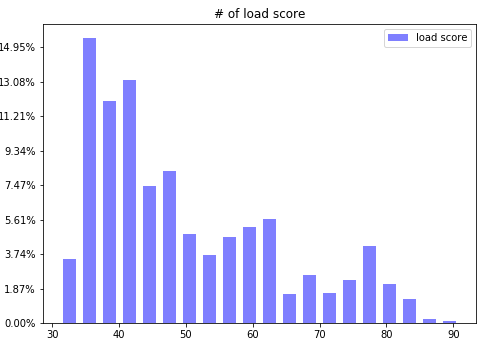
\includegraphics[width=4in]{histograph_of_load_scores.png}
\subsection*{load levels 分布}
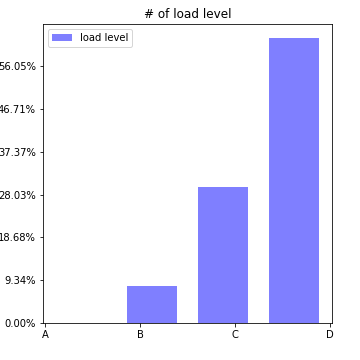
\includegraphics[width=3in]{histograph_of_load_levels.png}
\subsection*{performance scores 分布}
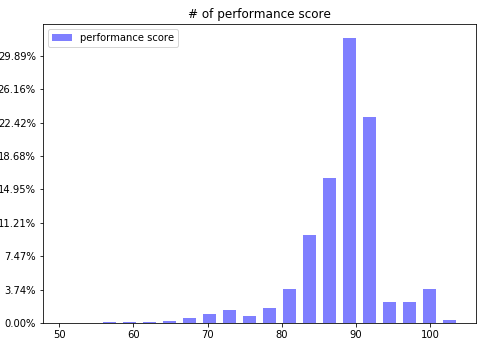
\includegraphics[width=4in]{histograph_of_perf_scores.png}
\subsection*{performance levels 分布}
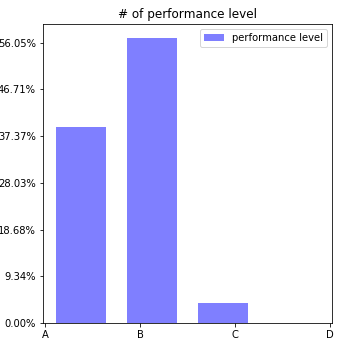
\includegraphics[width=3in]{histograph_of_perf_levels.png}

\section*{选择的特征}
\subsection*{load选择特征(lasso/pearson/reliefF)}
\renewcommand{\arraystretch}{1.2}    
	\begin{tabular}{|c|c|c|c|c|c|c|c|c|}  
		\hline    
		\textbf{Feature} & 2080020 & 2080021 & 2080022 & 2080023 & 2080024 & 2080025 & 2080026 & 2080027   
		\\\hline  
		\textbf{Selected} &1       &1        &1        &1        &1        &1        &1        &1       
		\\\hline  
		\textbf{Feature} & 2080028 & 2080029 & 2080030 & 2080031 & 2080032 & 2080033 & 2080034 & \textbf{Aggregate(15)}  
		\\\hline  
		\textbf{Selected} &1       &1        &1        &1        &1        &1        &1        &15/15   
		\\\hline   
	\end{tabular}  
	\vspace{1.5mm}  
\subsection*{performance选择特征(lasso/pearson/reliefF)}
\renewcommand{\arraystretch}{1.2}    
\begin{tabular}{|c|c|c|c|c|c|c|c|c|}  
	\hline    
	\textbf{Feature} & 2080040 & 2080041 & 2080042 & 2080043 & 2080044 & 2080045 & 2080046 & 2080047   
	\\\hline  
	\textbf{Selected} &1       &1        &1        &1        &1        &1        &1        &1       
	\\\hline  
	\textbf{Feature} & 2080048 & 2080049 & 2080050 & 2080051 & 2080052 & 2080053 & 2080054 & 2080055  
	\\\hline  
	\textbf{Selected} &1       &1        &1        &1        &1        &1        &1        &1   
	\\\hline 
	\textbf{Feature} & 2080056 & 2080057 & 2080058 & 2080059 & 2080060 & 2080061 & 2080062 & 2080063
	\\\hline  
	\textbf{Selected} &1       &1        &1        &1        &1        &1        &1        & 1  
	\\\hline
	\textbf{Feature} & 2080064 & 2080065 & \textbf{Aggregate(26)} &        &         &         &      &
	\\\hline  
	\textbf{Selected} &1       &1        &26/26    &          &         &         &        &   
	\\\hline    
\end{tabular}  
\vspace{1.5mm} 

\section*{回归结果}
\subsection*{load 回归}
\renewcommand{\arraystretch}{1.5} %控制行高  
\begin{table}[!h]  
	\centering  
	\fontsize{6.5}{8}\selectfont  
	\begin{threeparttable}  
		\label{tab:performance_comparison}  
		\begin{tabular}{ccccccccc}  
			\toprule  
			\multirow{2}{*}{Method}&  
			\multicolumn{2}{c}{None}&\multicolumn{2}{c}{lasso}&\multicolumn{2}{c}{pearson}&\multicolumn{2}{c}{reliefF}\cr  
			\cmidrule(lr){2-3} \cmidrule(lr){4-5} \cmidrule(lr){6-7} \cmidrule(lr){8-9}
			&MSE&R2 score&MSE&R2 score&MSE&R2 score&MSE&R2 score\cr  
			\midrule  
			linearR&1.2747&0.9442&0.2367&0.9549&1.2094&0.9816&1.2162&0.9750\cr  			logisticR&0.9498&0.9799&0.9652&0.9790&0.9995&0.9780&0.9688&0.9785\cr  
			MLP&2.9818&0.7983&3.1836&0.7389&3.0546&0.7875&2.8714&0.8034\cr  
			\bottomrule  
		\end{tabular}  
	\end{threeparttable}  
\end{table}   
\subsection*{performance 回归}
\renewcommand{\arraystretch}{1.5} %控制行高  
\begin{table}[!h]  
	\centering  
	\fontsize{6.5}{8}\selectfont  
	\begin{threeparttable}  
		\label{tab:performance_comparison}  
		\begin{tabular}{ccccccccc}  
			\toprule  
			\multirow{2}{*}{Method}&  
			\multicolumn{2}{c}{None}&\multicolumn{2}{c}{lasso}&\multicolumn{2}{c}{pearson}&\multicolumn{2}{c}{reliefF}\cr  
			\cmidrule(lr){2-3} \cmidrule(lr){4-5} \cmidrule(lr){6-7} \cmidrule(lr){8-9}
			&MSE&R2 score&MSE&R2 score&MSE&R2 score&MSE&R2 score\cr  
			\midrule  
			linearR&1.2739&0.8762&1.2052&0.9829&1.2936&0.6281&1.2056&0.9758\cr  
			logisticR&3.1290&0.7582&2.8272&0.8252&3.0170&0.7928&2.8826&0.8097\cr  
			MLP&3.1290&0.7582&2.8272&0.8252&3.0170&0.7928&2.8826&0.8097\cr  
			\bottomrule  
		\end{tabular}  
	\end{threeparttable}  
\end{table}  

\section*{...}
\dots
 
\section*{分类结果}
\subsection*{load 分类}
\renewcommand{\arraystretch}{1.5} %控制行高  
\begin{table}[!h]  	
	\centering  
	\fontsize{5}{5}\selectfont  
	\begin{threeparttable}  
		\label{tab:performance_comparison}  
		\begin{tabular}{ccccccccccccc}  
			\toprule  
			\multirow{2}{*}{Method}&  
			\multicolumn{3}{c}{None}&\multicolumn{3}{c}{lasso}&\multicolumn{3}{c}{pearson}&\multicolumn{3}{c}{reliefF}\cr  
			\cmidrule(lr){2-4} \cmidrule(lr){5-7}\cmidrule(lr){8-10}\cmidrule(lr){11-13}  
			&Precision&Recall&F1-Measure&Precision&Recall&F1-Measure&Precision&Recall&F1-Measure&Precision&Recall&F1-Measure\cr  
			\midrule  
			SVM&0.9688&0.9680&0.9684&0.9670&0.9688&0.99679&0.9629&0.9649&0.9639&0.9651&0.9637&0.99644\cr  
			RF&0.9801&0.9773&0.9790&0.9762&0.9770&0.9766&0.9750&0.9730&0.9740&0.9821&0.9773&0.9797\cr  
			MLPC&0.9547&0.9548&0.9547&0.9600&0.9606&0.9603&0.9579&0.9547&0.9563&0.9580&0.9598&0.9589\cr  
			\bottomrule  
		\end{tabular}  
	\end{threeparttable}
\end{table} 
  
\subsection*{performance 分类}
\renewcommand{\arraystretch}{1.5} %控制行高  
\begin{table}[!h]  	
	\centering  
	\fontsize{5}{5}\selectfont  
	\begin{threeparttable}  
		\label{tab:performance_comparison}  
		\begin{tabular}{ccccccccccccc}  
			\toprule  
			\multirow{2}{*}{Method}&  
			\multicolumn{3}{c}{None}&\multicolumn{3}{c}{lasso}&\multicolumn{3}{c}{pearson}&\multicolumn{3}{c}{reliefF}\cr  
			\cmidrule(lr){2-4} \cmidrule(lr){5-7}\cmidrule(lr){8-10}\cmidrule(lr){11-13}  
			&Precision&Recall&F1-Measure&Precision&Recall&F1-Measure&Precision&Recall&F1-Measure&Precision&Recall&F1-Measure\cr  
			\midrule  
			SVM&0.9208&0.9283&0.9245&0.9184&0.9223&0.9203&0.6822&0.6919&0.6869&0.9206&0.9293&0.9249\cr  
			RF&0.9333&0.9443&0.9385&0.99313&0.9464&0.9386&0.9248&0.9422&0.93318&0.9356&0.9455&0.9404\cr  
			MLPC&0.9132&0.9249&0.9189&0.9113&0.9138&0.9125&0.9109&0.9265&0.9184&0.9150&0.9366&0.9253\cr  
			\bottomrule  
		\end{tabular}  
	\end{threeparttable}
\end{table}  

\end{document}